%Title: Literature studies for I262
%Author: A. Raggio
%Year: 2020

\documentclass[10pt]{beamer}

%
%Setting file
%

\usepackage[T1]{fontenc}
\usepackage[utf8]{inputenc}

\usepackage[english]{babel}

\usepackage{graphicx}
\graphicspath{{images/}}
\usepackage{float}
\usepackage{tikz}
\usepackage{caption}
\usepackage{subcaption}

\usetheme{default}
\usefonttheme{structurebold}


% ---------------------------------
% color definitions
\usepackage{color}
% \definecolor{LISA_BLUE}{rgb}{0.25,0.33,0.66}
\definecolor{LISA_BLUE}{cmyk}{0.99,0.88,0.29,0.18}

\setbeamercolor{normal text}{fg=LISA_BLUE}
\setbeamercolor{frametitle}{fg=LISA_BLUE}

\newcommand\insertlocation{}  % Empty by default.
\newcommand\location[1]{\renewcommand\insertlocation{#1}}

\newcommand\insertperiod{}  % Empty by default.
\newcommand\period[1]{\renewcommand\insertperiod{#1}}



\setbeamertemplate{itemize items}[circle]
\setbeamercolor{title}{fg=white}



%-----------------------------------------Title page settings-----------------------------------------%
\title{\normalsize }

\institute{}

\author{}


\date{}
\titlegraphic{% 
\vspace{0.05\textheight}
	\centering
	
\includegraphics[height=3cm]{jyu-keskitetty-kaksikielinen.eps}\\
\vspace{-0.03\textheight}
}
%-----------------------------------------Title page settings-----------------------------------------%


\setbeamertemplate{footline}
{
 \begin{beamercolorbox}{section in head/foot}
 \vskip2pt\hspace{0.095cm} Andrea Raggio \hfill Jyv\"{a}skyl\"{a} - 2021 \hspace{0.15cm}\phantom{x}\vskip2pt
 \end{beamercolorbox}%
}


\begin{document}
\frame{\titlepage}
\begin{frame}{Production XS}	
	\centering
	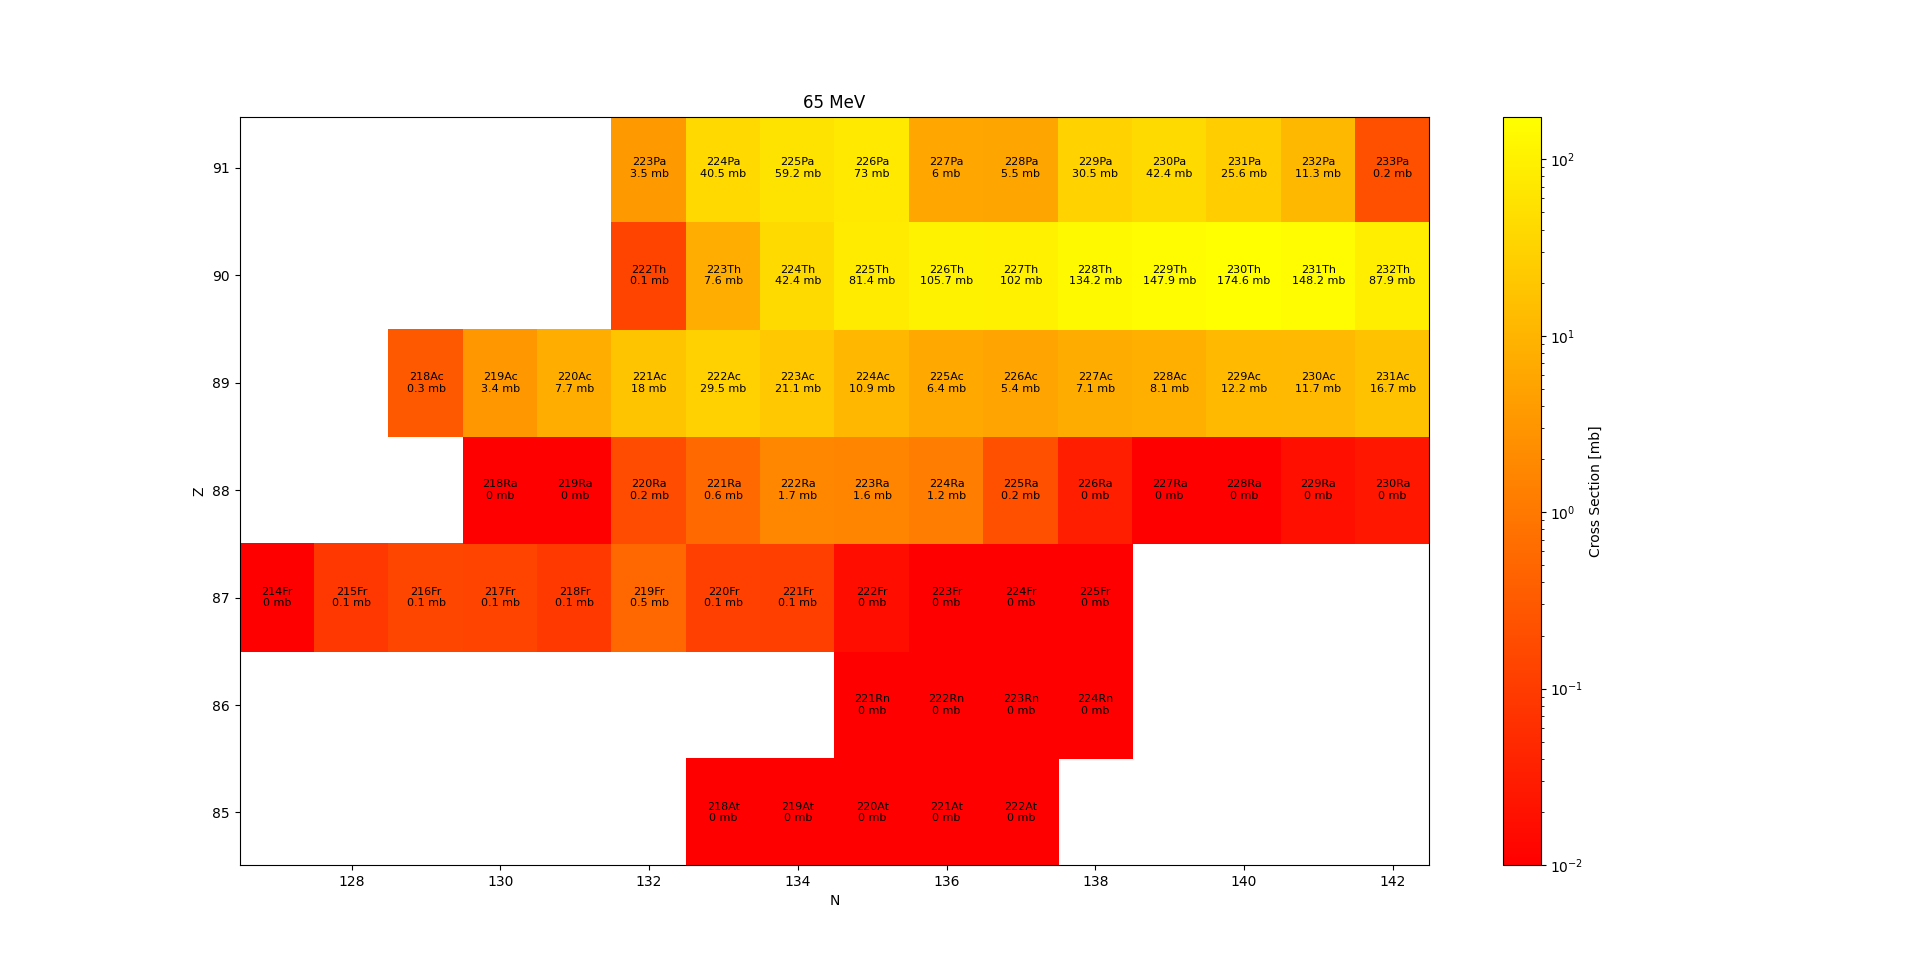
\includegraphics[width=1.2\textwidth]{Segre.png}

\end{frame}
\begin{frame}{Even Mass Scan}	
	\begin{columns}
		\begin{column}{0.5\textwidth}
			\begin{overlayarea}{\textwidth}{0.5\textheight}
				\centering
				\textcolor{red}{\textbf{MASS 226} (II)}\\
				%\vspace{0.05\textheight}
				{\footnotesize $^{226}$Th~(105~mb) $^{226}$Pa~(73~mb) \textcolor{red}{$^{226}$Ac~(5~mb)}}\\
				\vspace{0.05\textheight}
				\textcolor{red}{\textbf{MASS 222} (I)}\\
				{\footnotesize\textcolor{red}{$^{222}$Th~(0.1~mb)} $^{222}$Ac~(30~mb) $^{222}$Ra~(1.7~mb) }\\
				\vspace{0.05\textheight}
				\textcolor{red}{\textbf{MASS 218} (III)}\\
				{\footnotesize\textcolor{red}{$^{218}$Ac~(0.3~mb)} $^{218}$Fr~(0.1~mb*) $^{218}$Rn~(*) }
			\end{overlayarea}
		\end{column}
		\begin{column}{0.5\textwidth}
			\begin{overlayarea}{\textwidth}{0.5\textheight}
				\centering
				\textcolor{red}{\textbf{MASS 224} (I)}\\
				%\vspace{0.05\textheight}
				{\footnotesize \textcolor{red}{$^{224}$Pa~(40.5~mb)} $^{224}$Th~(42.4~mb) $^{224}$Ac~(11~mb) $^{224}$Ra~(1.2~mb)}\\
				\vspace{0.05\textheight}
				\textcolor{red}{\textbf{MASS 220} (II)}\\
				{\footnotesize\textcolor{red}{$^{220}$Ac~(7.7~mb)} $^{220}$Ra~(0.2~mb *) \textcolor{red}{$^{220}$Fr~(0.1~mb)} $^{220}$Rn~(*)}\\
			\end{overlayarea}
		\end{column}
	\end{columns}	
\end{frame}

\begin{frame}{Even Mass Scan}	
	\begin{columns}
		\begin{column}{0.5\textwidth}
			\begin{overlayarea}{\textwidth}{0.5\textheight}
				\centering
				\textcolor{red}{\textbf{MASS 226} (II)}\\
				%\vspace{0.05\textheight}
				{\footnotesize $^{226}$Th~(105~mb) $^{226}$Pa~(73~mb) \textcolor{green}{$^{226}$Ac~(5~mb)} Decay 83\% to $^{226}$Th}\\
				\vspace{0.05\textheight}
				\textcolor{red}{\textbf{MASS 222} (I)}\\
				{\footnotesize\textcolor{green}{$^{222}$Th~(0.1~mb)} $^{222}$Ac~(30~mb) $^{222}$Ra~(1.7~mb) }\\
				\vspace{0.05\textheight}
				\textcolor{red}{\textbf{MASS 218} (III)}\\
				{\footnotesize\textcolor{green}{$^{218}$Ac~(0.3~mb)} $^{218}$Fr~(0.1~mb*) $^{218}$Rn~(*) }
			\end{overlayarea}
		\end{column}
		\begin{column}{0.5\textwidth}
			\begin{overlayarea}{\textwidth}{0.5\textheight}
				\centering
				\textcolor{red}{\textbf{MASS 224} (I)}\\
				%\vspace{0.05\textheight}
				{\footnotesize $^{224}$Pa~(40.5~mb) $^{224}$Th~(42.4~mb) $^{224}$Ac~(11~mb) $^{224}$Ra~(1.2~mb)}\\
				\vspace{0.05\textheight}
				\textcolor{red}{\textbf{MASS 220} (II)}\\
				{\footnotesize\textcolor{red}{$^{220}$Ac~(7.7~mb)} $^{220}$Ra~(0.2~mb *) \textcolor{red}{$^{220}$Fr~(0.1~mb)} $^{220}$Rn~(*)}\\
			\end{overlayarea}
		\end{column}
	\end{columns}	
\end{frame}

% \begin{frame}{MASS 226}	
% 	\begin{columns}
% 		\begin{column}{0.5\textwidth}
% 			\begin{overlayarea}{\textwidth}{0.5\textheight}
% 				\centering
% 				\vspace{-0.2\textheight}
% 				\textcolor{red}{\textbf{$^{226}$Th}}\\
% 				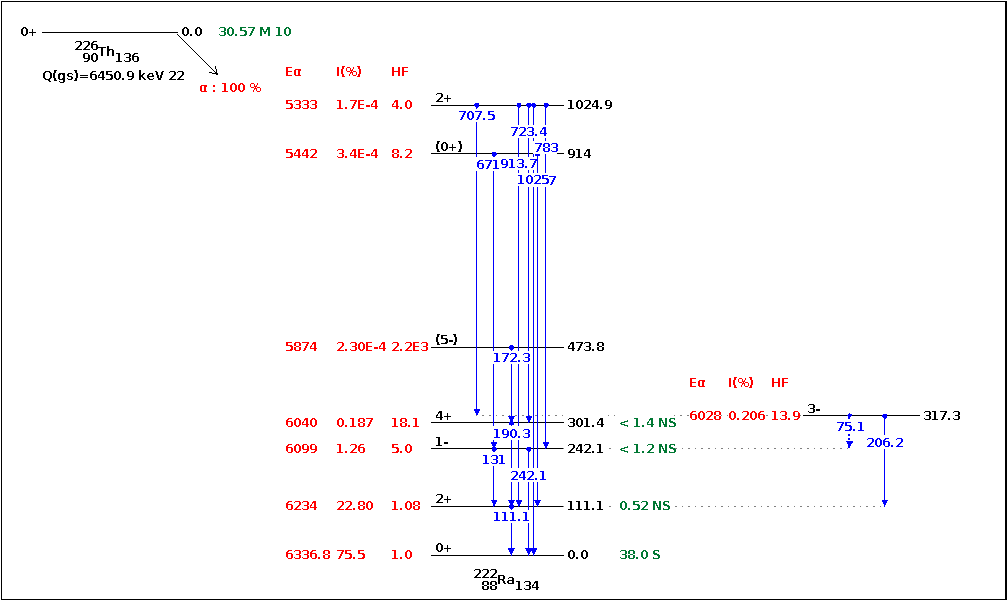
\includegraphics[width=\textwidth]{226Th.png}
% 				\tiny{Luca, A. (2020). 226Th nuclear decay data evaluation. Applied Radiation and Isotopes, 155, 108941.}\\
% 				\vspace{0.05\textheight}
% 				\textcolor{red}{Half-Life measurement}\\
% 				\tiny{Pommé, S., et al. "Measurement of the 226Th and 222Ra half-lives." Applied Radiation and Isotopes 70.9 (2012): 1913-1918.}\\
% 				\vspace{0.05\textheight}
% 				\tiny{
% 				$\gamma \gamma$ : see 1976Ku08, 1956As38.\\
% 				$\alpha \gamma$ : see 1963Le17, 1969Pe17, 1969Br10.\\}
% 			\end{overlayarea}
% 		\end{column}
% 		\begin{column}{0.5\textwidth}
% 			\begin{overlayarea}{\textwidth}{0.5\textheight}
% 				\centering
% 				\vspace{-0.2\textheight}
% 				\textcolor{red}{\textbf{$^{226}$Pa}}\\
% 				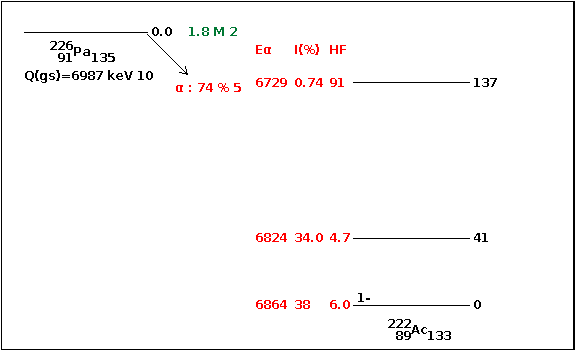
\includegraphics[width=0.98\textwidth]{226Pa.png}
% 				\tiny{Nuclear Data Sheets 112,2851 (2011)}\\
% 				\vspace{0.05\textheight}
% 				\tiny{
% 				$\alpha$ : see 1992Wo14 (+1964Mc21, 1991Ry01, 1951Me10, 1968Ha14, 1988Hu08)}\\
% 			\end{overlayarea}
% 		\end{column}
% 	\end{columns}	
% \end{frame}

% \begin{frame}{MASS 222}	
% 	\begin{columns}
% 		\begin{column}{0.5\textwidth}
% 			\begin{overlayarea}{\textwidth}{0.5\textheight}
% 				\centering
% 				\vspace{-0.2\textheight}
% 				\textcolor{red}{\textbf{$^{222}$Ra}}\\
% 				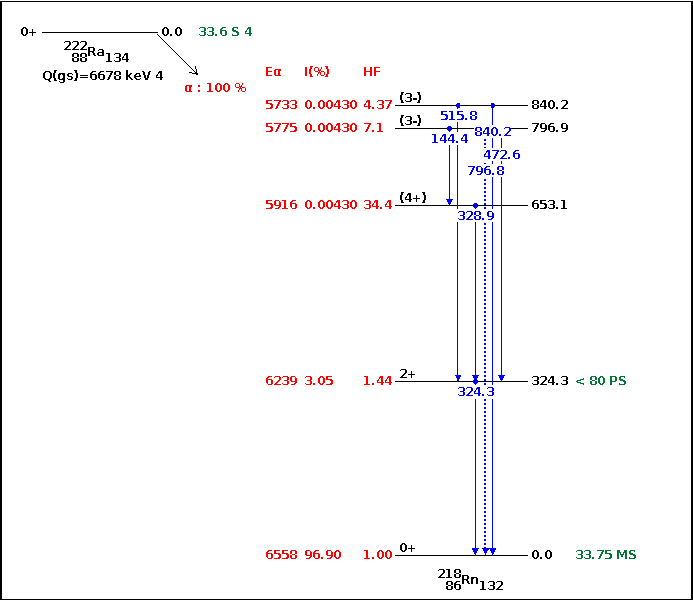
\includegraphics[width=0.7\textwidth]{222Ra.png}\\
% 				\tiny{Nuclear Data Sheets 160, 405 (2019)}\\
% 				\vspace{0.05\textheight}
% 				\tiny{
% 				T1/2 : see 2012Po13\\
% 				$\gamma \gamma$ : see 1960St20.\\
% 				$\alpha \gamma$ : see 1963Le17, 1969Pe17.\\}
% 			\end{overlayarea}
% 		\end{column}
% 		\begin{column}{0.5\textwidth}
% 			\begin{overlayarea}{\textwidth}{0.5\textheight}
% 				\centering
% 				\vspace{-0.2\textheight}
% 				\textcolor{red}{\textbf{$^{222}$Ac}}\\
% 				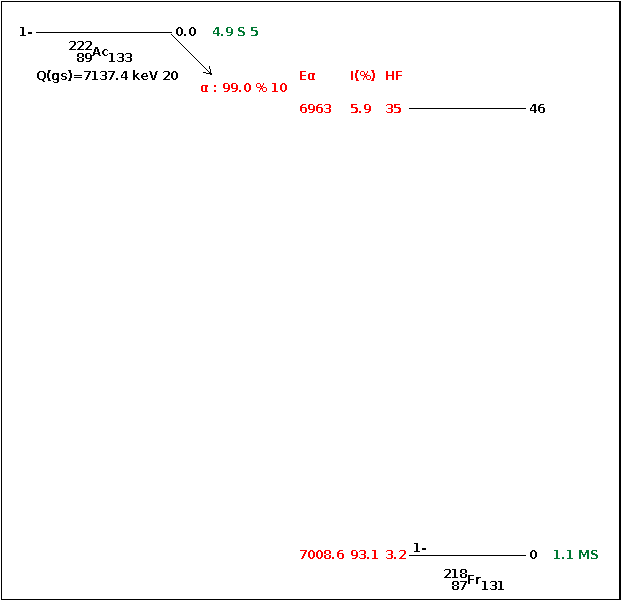
\includegraphics[width=0.64\textwidth]{222Ac.png}\\
% 				\tiny{Nuclear Data Sheets 160, 405 (2019)}\\
% 				\vspace{0.05\textheight}
% 				\tiny{
% 					ISOMERIC STATE 0.0+X (63s T1/2)\\
% 				T1/2 : see 1972Es03\\
% 				$\alpha$ : see 1972Es03}\\
% 			\end{overlayarea}
% 		\end{column}
% 	\end{columns}	
% \end{frame}

% \begin{frame}{Peak Fitting}
	
% 	\vspace{-0.1\textheight}
% 	\begin{columns}
% 		\begin{column}{0.5\textwidth}
% 			\begin{overlayarea}{\textwidth}{0.5\textheight}
% 				\centering
% 				\vspace{-0.05\textheight}
% 				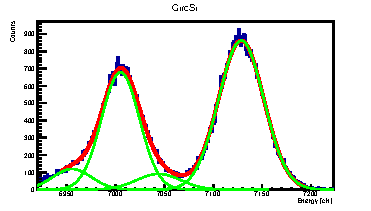
\includegraphics[width=0.95\textwidth]{Circ_Si_full.pdf}
% 				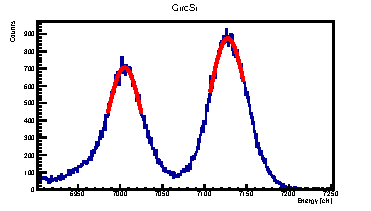
\includegraphics[width=0.95\textwidth]{Circ_Si_top.pdf}
% 			\end{overlayarea}
% 		\end{column}
% 		\begin{column}{0.5\textwidth}
% 			\begin{overlayarea}{\textwidth}{0.5\textheight}
% 				\centering
% 				\vspace{-0.05\textheight}
% 				\includegraphics[width=0.95\textwidth]{SiLi_full.pdf}
% 				\includegraphics[width=0.95\textwidth]{SiLi_top.pdf}
% 			\end{overlayarea}
% 		\end{column}
% 	\end{columns}	



% \end{frame}

% \begin{frame}{Calibration Fitting}
	

% 	\centering
% 	\vspace{-0.05\textheight}
% 	\textbf{Two Fitting methods $\rightarrow$ Pol1 - Pol2}  
% 	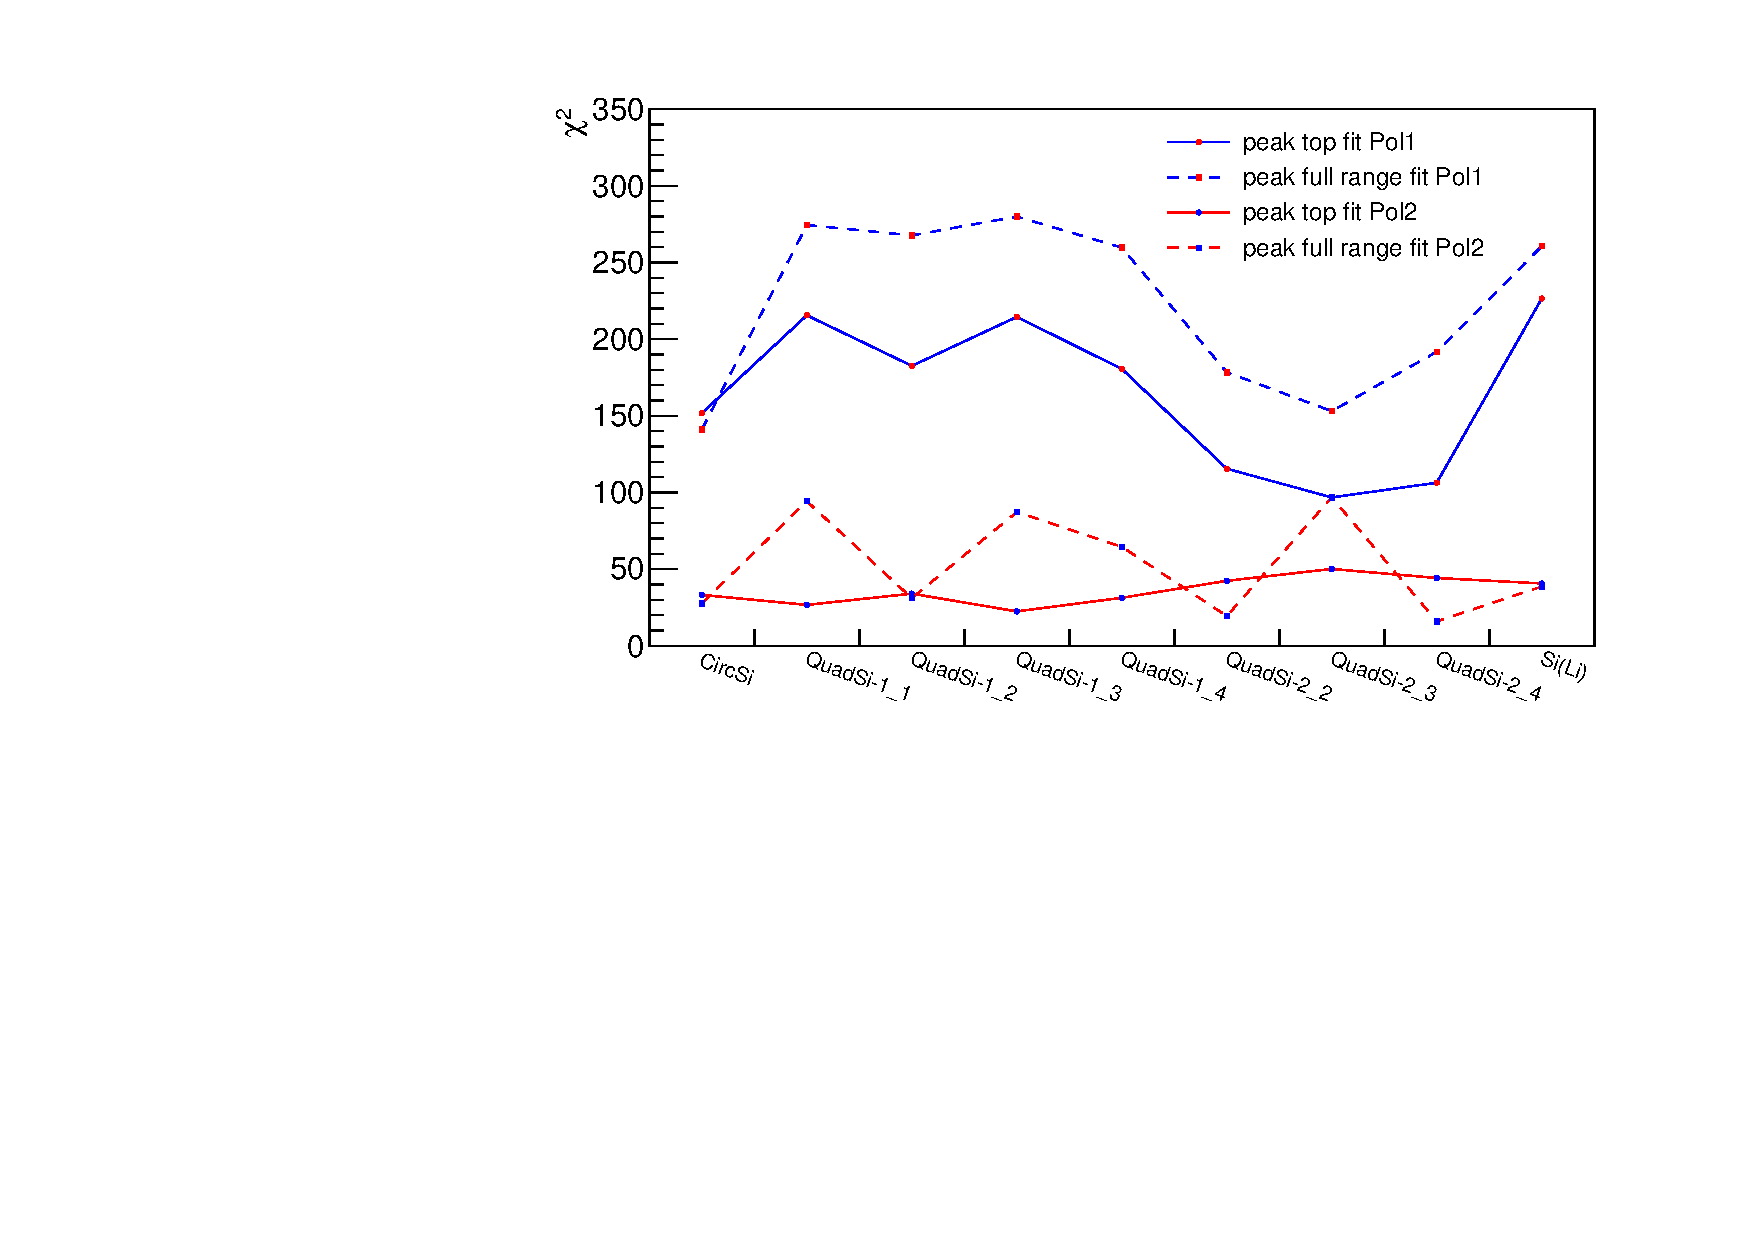
\includegraphics[width=0.85\textwidth]{Chi_comparison.pdf}




% \end{frame}

% \begin{frame}{Calibration Fitting}
	
% 	\vspace{-0.2\textheight}
% 	\begin{columns}
% 		\begin{column}{0.5\textwidth}
% 			\begin{overlayarea}{\textwidth}{0.5\textheight}
% 				\centering
% 				\vspace{-0.05\textheight}
% 				\tiny Pol1 Fit\\
% 				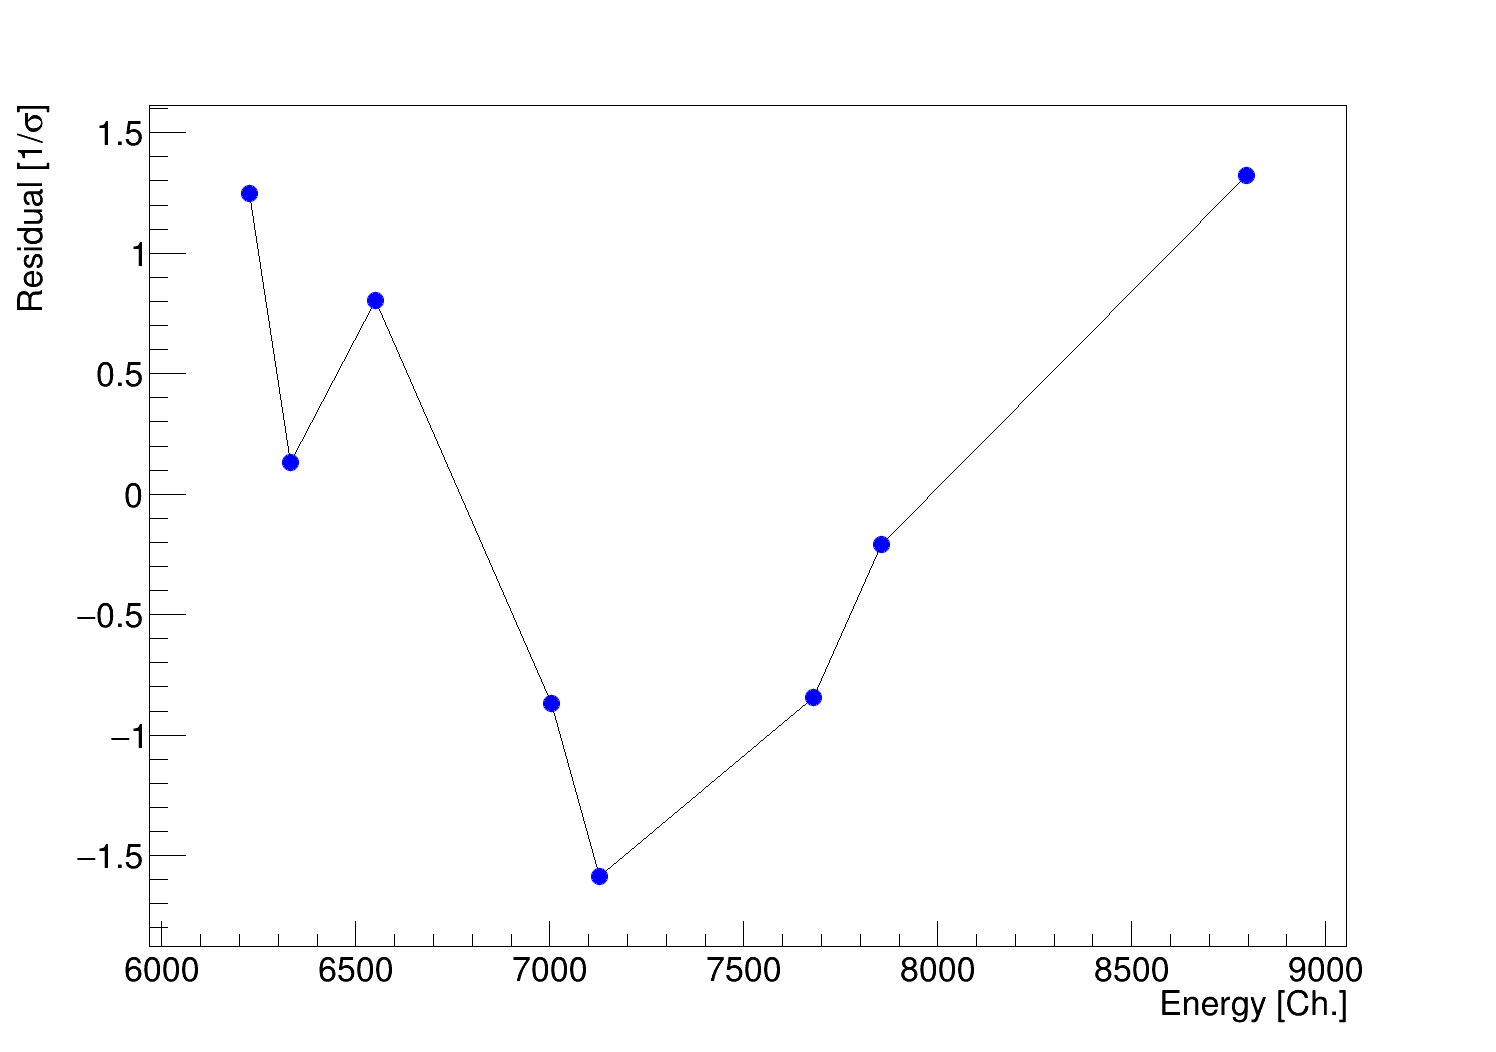
\includegraphics[width=0.85\textwidth]{CircSi_fitting1_LinearCal.png}\\
% 				Pol2 Fit\\
% 				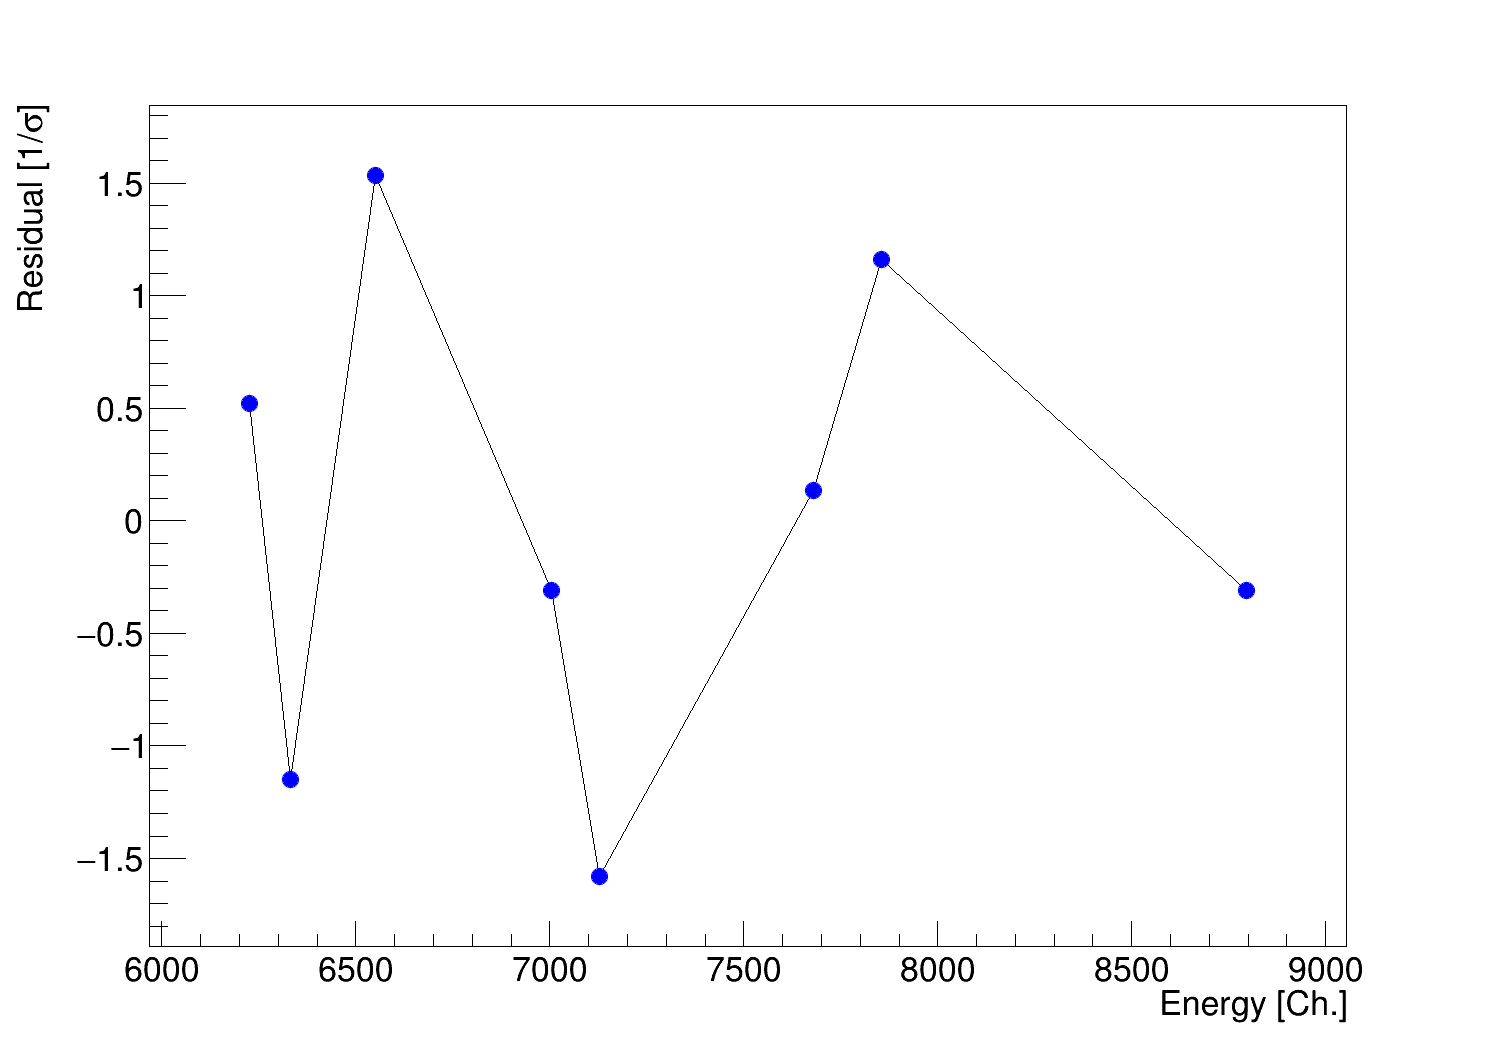
\includegraphics[width=0.85\textwidth]{CircSi_fitting1_Pol2Cal.png}
% 			\end{overlayarea}
% 		\end{column}
% 		\begin{column}{0.5\textwidth}
% 			\begin{overlayarea}{\textwidth}{0.5\textheight}
% 				\centering
% 				\vspace{-0.05\textheight}
% 				\tiny Pol1 Fit\\
% 				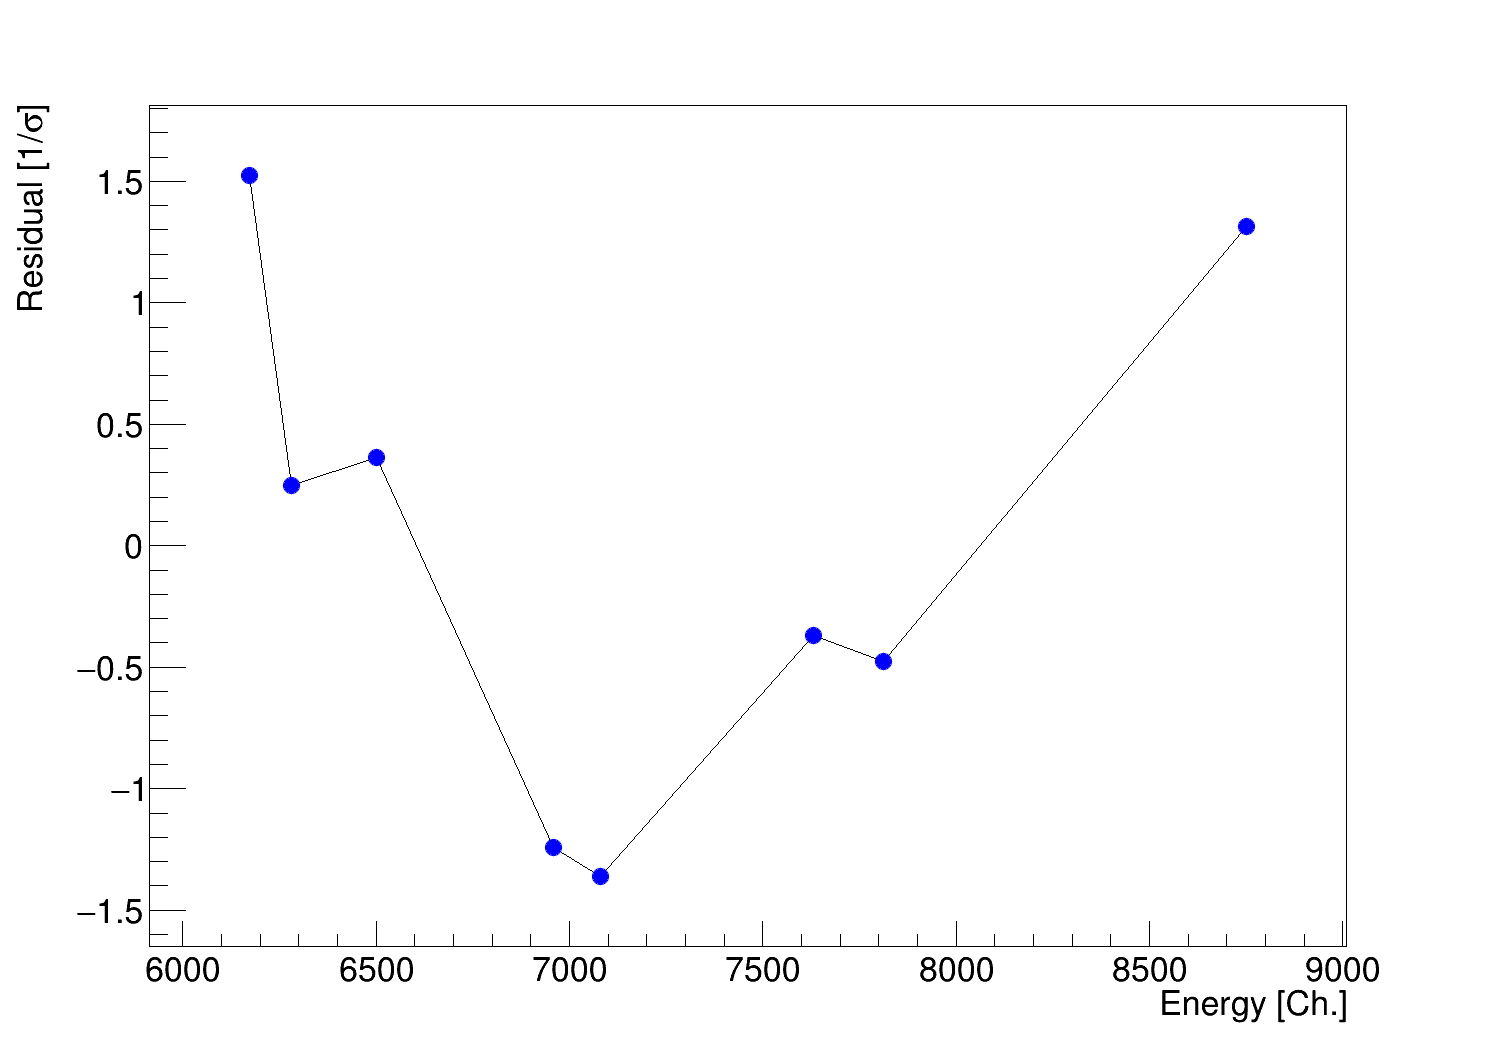
\includegraphics[width=0.85\textwidth]{Si(Li)_fitting1_LinearCal.png}\\
% 				Pol2 Fit\\
% 				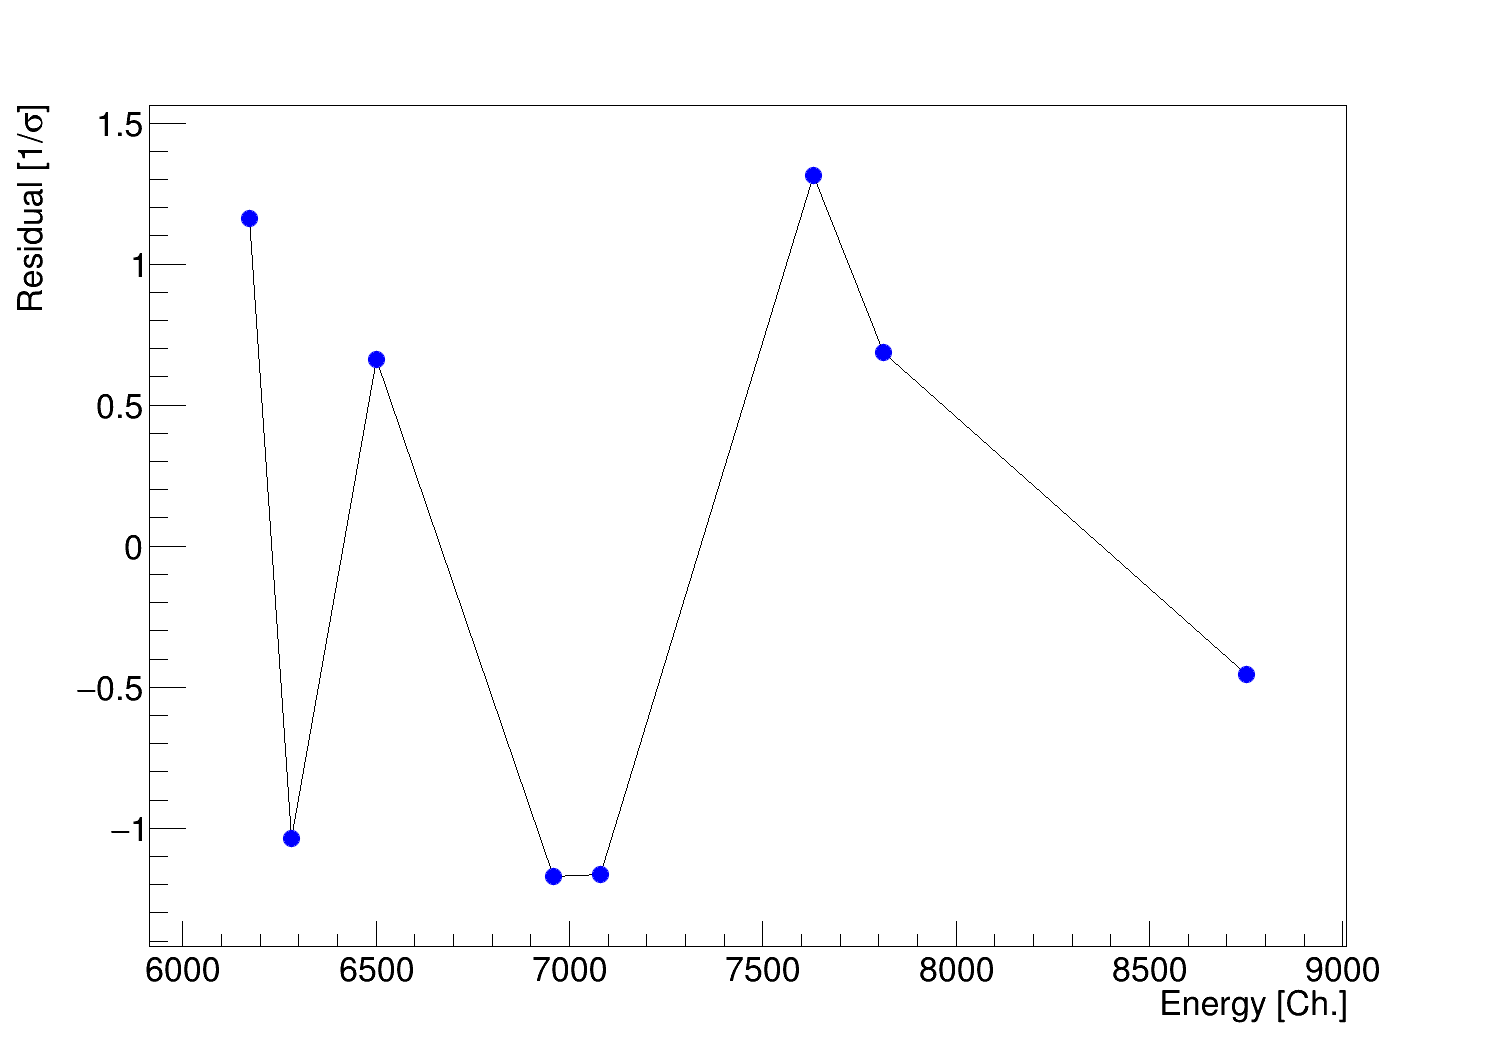
\includegraphics[width=0.85\textwidth]{Si(Li)_fitting1_Pol2Cal.png}
% 			\end{overlayarea}
% 		\end{column}
% 	\end{columns}	


% \end{frame}


% \begin{frame}{Low Energy Problem?}
% 	\centering
% 	\vspace{-0.2\textheight}
% 	Inside the energy range 6000 keV - 9000 keV\\ the two calibration are in good agreement.\\
% 	\vspace{0.1\textheight}
% 	\textbf{LOW ENERGY?}\\
% 	Event at 214~ch. in SiLi detector $\rightarrow$ $\sim$253~keV (Pol1) - $\sim$621~keV (Pol2)

% \end{frame}

% \begin{frame}{Event Builder}
% 	\centering
% 	\vspace{-0.2\textheight}
	
% 	\only<1>{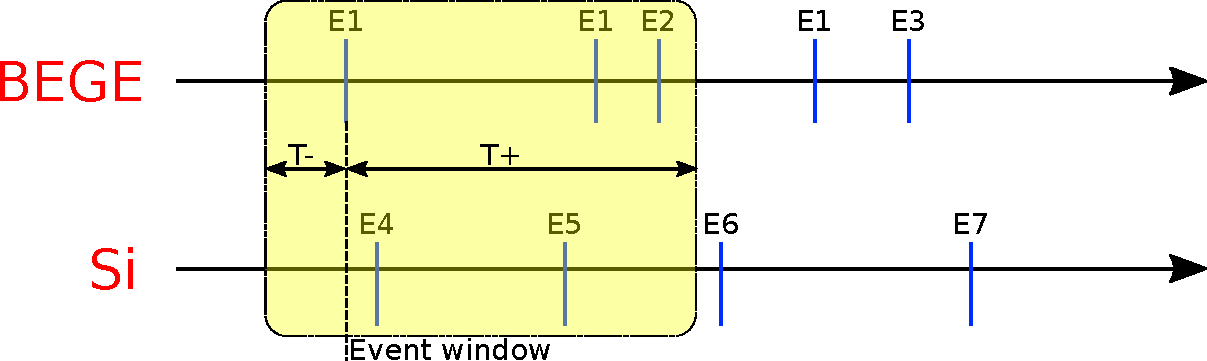
\includegraphics[width=0.85\textwidth]{Event_0.pdf}}%
% 	\only<2>{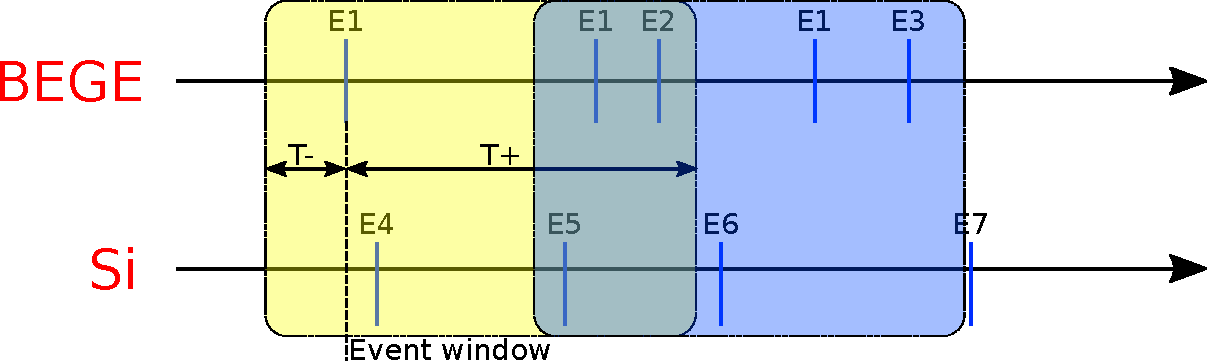
\includegraphics[width=0.85\textwidth]{Event_1.pdf}}%
% 	\only<3>{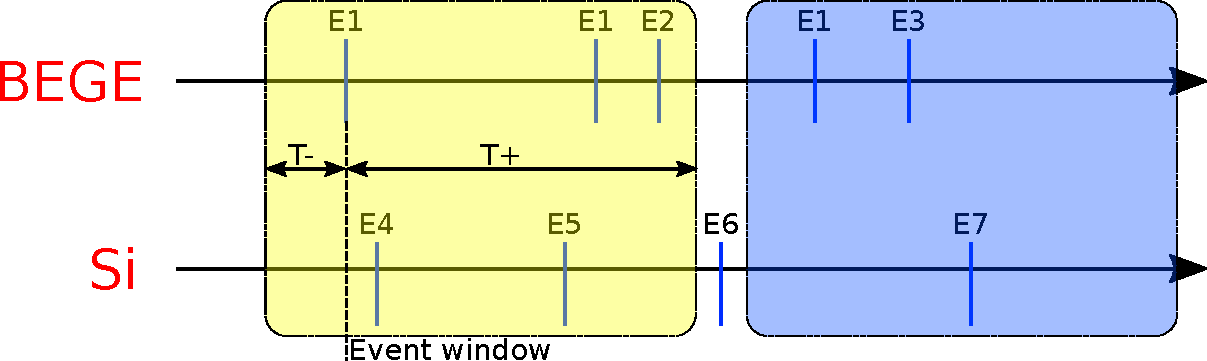
\includegraphics[width=0.85\textwidth]{Event_2.pdf}}%

% 	\vspace{0.1\textheight}
% 	\textbf{E1 is the trigger}
% \end{frame}

\end{document}